\section{Queue-Detektion}

Wie schon in der Einleitung beschrieben, soll es dem Spieler möglich sein, mit dem realen Queue die simulierten Kugeln zu stoßen.
Dazu wird das Spielfeld, und somit auch der Queue, von einer Kamera erfasst. 
Um die Interaktion des Queues mit den Kugeln zu ermöglichen, muss in dem Eingabebild der Kamera der Queue, bzw. die für die Kollisionsberechnung relevanten Punkte, extrahiert werden.

In den folgenden Abschnitten wird dazu eine Möglichkeit beschrieben, welche zunächst mittels eines Schwellwertverfahrens den Queue vom Hintergrund segmentiert.
Basierend auf dem segmentierten Bild wird dann unter Verwendung der Hauptkomponentenanalyse ein Kollisionspunkt ermittelt.
Schließlich wird die Einbindung des Kollisionspunktes in die Kollisionsberechnung erläutert, welche die Detektion des Queues abschließt.

\subsection{Segmentierung}
Sei $\textbf{I} \in \{0, \dots, 255\}^{n \times m \times 3}$ das von der Kamera aufgenommene $n \times m$ große RGB-Farbbild.
Ziel der Segmentierung ist es, ein Binärbild $\textbf{B} \in \{0,1\}^{n \times m}$ zu erzeugen, welches die Pixel im Eingabebild charakterisiert, die dem Queue zugeordnet werden.

Da der Queue mit einer schwarzen Farbe lackiert wurde, wird dies mithilfe eines Schwellwertverfahrens basierend auf dem Farbwert der Pixel bewerktstelligt.
Das im RGB-Farbraum vorliegende Eingabebild $\textbf{I}$ wird dazu zunächst in den HSV-Farbraum überführt. 
Im HSV-Farbraum wird ein Farbwert mit seinem Farbton $H \in [0, 360]$, Sättigung $S \in [0, 1]$ und Helligkeitswert $V \in [0, 1]$ dargestellt (s. Abb. 3.6).

\begin{figure}[H]
	\label{fig:HSVRGB}
	\subfigure[]{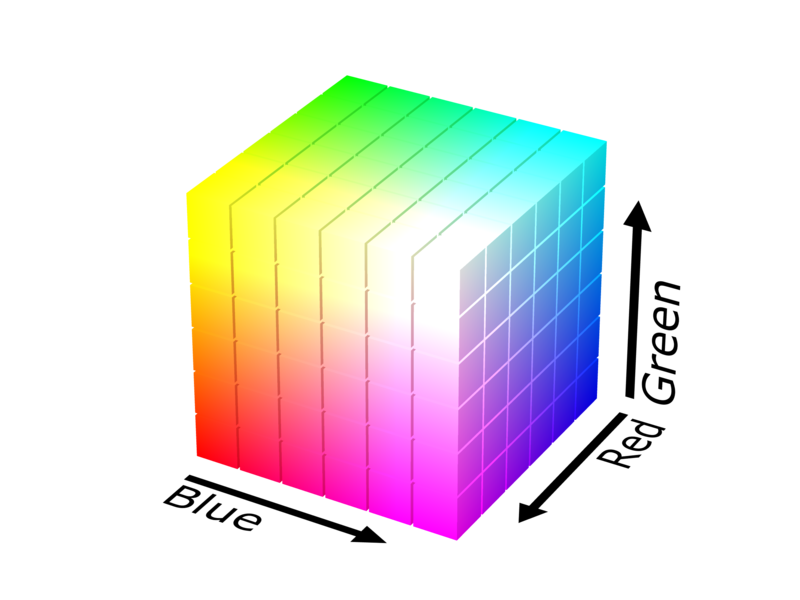
\includegraphics[height=3.3cm]{bilder/rgb.png}\label{fig:RGB}}
	\subfigure[]{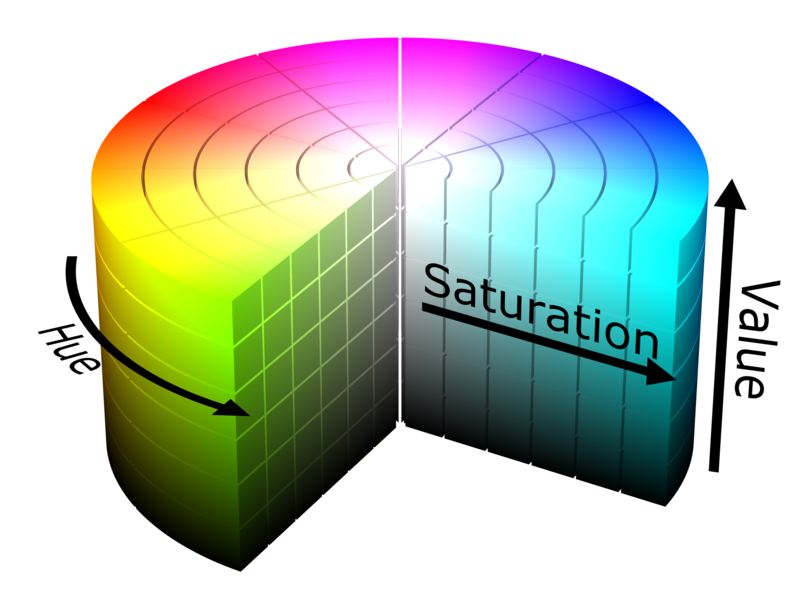
\includegraphics[height=3.0cm]{bilder/hsv.png}\label{fig:HSV}}
	\centering
	\caption{Darstellung von Farbtönen im (a) RGB-Farbraumes durch Rot-, Grün- und Blauanteileund und  im (b) HSV-Farbraumes durch Farbton (Hue), Sättigung (Saturation) und Helilgkeitswert (Value). Dunkle Farben im HSV-Farbraum haben einen kleinen Helligkeitswert.}
\end{figure}

Dies ermöglicht es, lediglich einen Schwellwert $\theta$ für den Helligkeitswert festzulegen, um den schwarzen Anteil des Bildes und damit den Queue zu segmentieren. 
Für das transformierte Bild $\textbf{I}_{HSV}$ ergibt sich die Berechnung des Wertes von $\textbf{B}$ an der Stelle $i, j$ für einen Schwellwert $\theta$ somit durch folgende Formel:
\begin{equation*}
\textbf{B}[i,j] = \begin{cases}
1 &\text{, falls $\textbf{I}_{HSV}[i, j, 3] \leq \theta$}\\
0 &\text{sonst}
\end{cases}
\end{equation*}

Durch die unterschiedliche Beleuchtung des Queues ergeben sich in dem entstehenden Binärbild größere Lücken, die die weitere Erkennung des Queues beeinflussen würden.
Um dies zu verhindern, werden mittels eines morphologischen Closings diese Lücken gefüllt.
Bei einem morphologischen Closing wird zunächst eine Dilatation und dann eine Erosion auf dem Bild mit durch ein $k \times k$ großes, rechteckiges Fenster durchgeführt. 
Für die Dilatation wird dem Fenster über das Bild gelaufen und dabei der zentrale Pixel des Fensters auf den maximalen Wert im Fenster gesetzt.
Analog dazu wird bei der Erosion der Wert des zentralen Pixels auf den minimalen Wert im Fenster gesetzt.
Insgesamt werden durch diese beiden Operationen die Lücken im Binärbild geschlossen.

\begin{figure}[H]
	\label{fig:thresholded}
	\subfigure[]{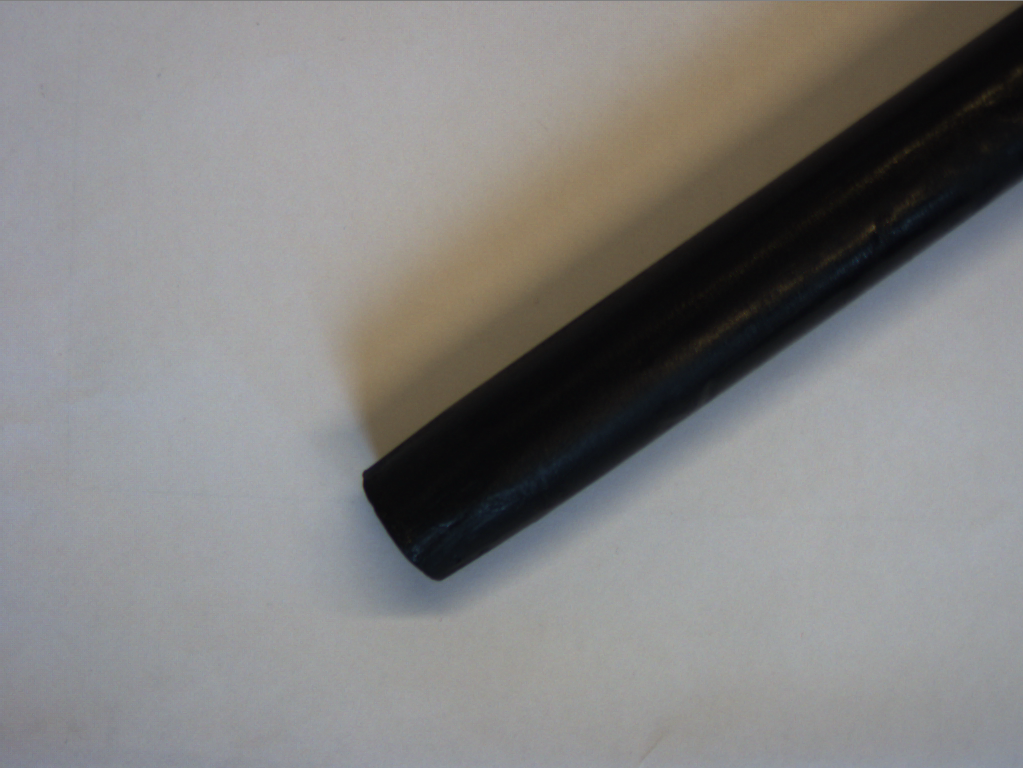
\includegraphics[height=3.3cm]{bilder/queue_orig.png}}
	\subfigure[]{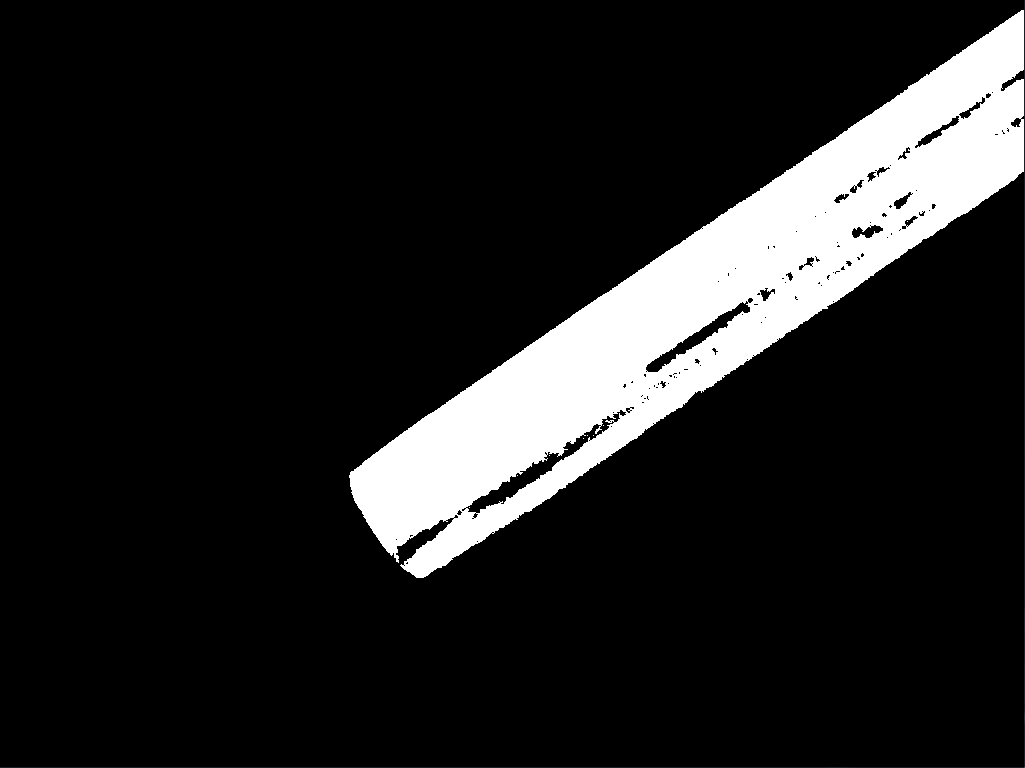
\includegraphics[height=3.3cm]{bilder/queue_thresholded.png}}
	\subfigure[]{
\includegraphics[height=3.3cm]{bilder/queue_close.png}}	
	\centering
	\caption{Ergebnis der Segmentierung des Eingabebildes. (a) Eingebild mit $1024 \times 768$ Pixeln, (b) Binärbild aus Schwellwertverfahren ($\theta = 30$),  (c) Ergebnis des morphologischen Closings ($k=15$)}
\end{figure}

\subsection{Erkennung des Kollisionspunktes}
Um nicht mit jedem im Binärbild als $\textbf{1}$ klassifizierten Punkt kollidieren zu müssen, wird nur mit der Spitze des Queues kollidiert.
Die Spitze des Queues wird dabei durch die Hauptkomponentenanalyse bestimmt.

Dazu werden zunächst die Koordinaten $i, j$ der Punkte aus $\textbf{B}$ mit $\textbf{B}[i,j] = 1$ als Zeilenvektoren in einer $l \times 2$ Matrix $\textbf{X}$ zusammengeführt.
Daraufhin wird der Mittelwert für beiden Dimensionen berechnet und die Koordinaten normalisiert:
\begin{equation*}
\textbf{u} = (u_1, u_2)\text{ mit }u_j = \frac{1}{k}\sum_{i=1}^{k}\textbf{X}_{i, j}, j \in \{1,2\}
\end{equation*}
\begin{equation*}
\textbf{A} = \textbf{B} - \textbf{h}\textbf{u}^T \text{ mit } \textbf{h}[i] = 1 \text{ für } i=1,\dots,l
\end{equation*}



Binärbild $\textbf{B} \in \{0, 1\}^{n\times m}$ Ausgabe der Segmentierung

Da der Queue 

Hauptkomponentenanalyse:

Koordinaten in $\textbf{B}$ der als Queue klassifizierten Pixel als Zeilenvektoren:

$X = \{(x, y) \mid \textbf{B}_{x,y} = 1, x \in [1,n], y \in [1,m]\}$, $k = |\textbf{B}|$

Sei $\textbf{X}$ die $k\times 2$ Matrix der $k$ Zeilenvektoren aus $X$

Berechnung des Mittelwertes für beide Dimensionen:

Normalisierung mittels des Mittelwertes:

$\textbf{A} = \textbf{B} - \textbf{h}\textbf{u}^{T}$ mit dem $k\times 1$ Spaltenvektor $\textbf{h}, h_i = 1$ für $i = 1,\dots,k$

Bestimmung der $2\times2$ Kovarianzmatrix:

$\textbf{C} = \frac{1}{k-1} {\textbf{B}}^{T} \cdot \textbf{B}$





\subsection{Bewegungsinterpolation und Kollisionsberechnung}





